%----------------------------------------------------------------------------------------
%	PACKAGES AND THEMES
%----------------------------------------------------------------------------------------
\documentclass[aspectratio=169,xcolor=dvipsnames]{beamer}
\usepackage[T1]{fontenc}
\usetheme{DarkConsoleFiraRemix}

\usepackage{hyperref}
\usepackage{graphicx} % Allows including images
\usepackage{booktabs} % Allows the use of \toprule, \midrule and \bottomrule in tables
\usepackage[natbib=true,style=authoryear,backend=bibtex,useprefix=true]{biblatex}
\addbibresource{references.bib}
\usepackage{multirow}
\usepackage{ulem}
\usepackage{caption} 

\setbeamercovered{invisible}

\graphicspath{ {../images/} } 

\newcommand\mperiod[0]{\;\;\;.}
\newcommand\mcomma[0]{\;\;\;,}

\AtBeginSection[]{
  \frame<beamer>{ 
    \frametitle{Outline}   
 
\tableofcontents[currentsection]}
}

%----------------------------------------------------------------------------------------
%	TITLE PAGE
%----------------------------------------------------------------------------------------

% The title
\title[short title]{Privacy-preserving Data Generation:}
\subtitle{Towards generating privacy-preserving, synthetic and useful time series ECG data for anomaly detection}
\author[SJTU]{Sijun John Tu}
\institute{KTH x RISE}
\date{\today} % Date, can be changed to a custom date


%----------------------------------------------------------------------------------------
%	PRESENTATION SLIDES
%----------------------------------------------------------------------------------------

\begin{document}

\begin{frame}
    % Print the title page as the first slide
    \titlepage
\end{frame}

\begin{frame}{Outline}
    % Throughout your presentation, if you choose to use \section{} and \subsection{} commands, these will automatically be printed on this slide as an overview of your presentation
    \tableofcontents
\end{frame}

\section{Project introduction}

\begin{frame}
    \frametitle{Machine Learning Pipeline}
    \tikz{
            \node[circle,fill=Button1,inner sep=3pt] (c) at (0,0){};
            \node[circle,fill=Button2,inner sep=3pt] (c) at (0.5,0){};
            \node[circle,fill=Button3,inner sep=3pt] (c) at (1,0){};
        }~~~~~~\textcolor{gold}{Figure: }High-level machine learning pipeline
    \begin{figure}[h]
        
        \centering
        \includegraphics[scale=0.45]{ml_pipeline.png}
    \end{figure}
\end{frame}



\begin{frame}{Anomaly detection using privacy-preserving, synthetic time series data}
    
    \begin{itemize}
        \item<1-> Problem
        \begin{itemize}
            \item<1-> ML models are very \alert{data hungry}.
            \item<1-> In many cases sharing data comes with \alert{privacy risks}.
        \end{itemize}
        \item<2-> Solution:
        \begin{itemize}
            \item<2-> Promising solution: \alert{synthetic data} with privacy guarantees!
            \item<2-> Synthetic data with \alert{differential private} (DP) guarantees is a promising solution to ensure privacy independent of downstream task.
        \end{itemize}
        \item<3-> BUT:
        \begin{itemize}
            \item<3-> \alert{Privacy-Utility-Tradeoff}: Commonly, a gain in privacy results in a loss of utility. 
            \item<3-> For \alert{anomaly detection} this might not be the case (?).
        \end{itemize}
    \end{itemize}
\end{frame}


\begin{frame}{Structure}
    
    \begin{figure}[h]
        \begin{flushleft}
            \tikz{
            \node[circle,inner sep=3pt] (c) at (-0.5,0){};
            \node[circle,fill=Button1,inner sep=3pt] (c) at (1.0,0){};
            \node[circle,fill=Button2,inner sep=3pt] (c) at (1.5,0){};
            \node[circle,fill=Button3,inner sep=3pt] (c) at (2.0,0){};
        }~~~~~~\textcolor{gold}{Figure: }Structure of Experiment pipeline
        \end{flushleft}
        \centering
        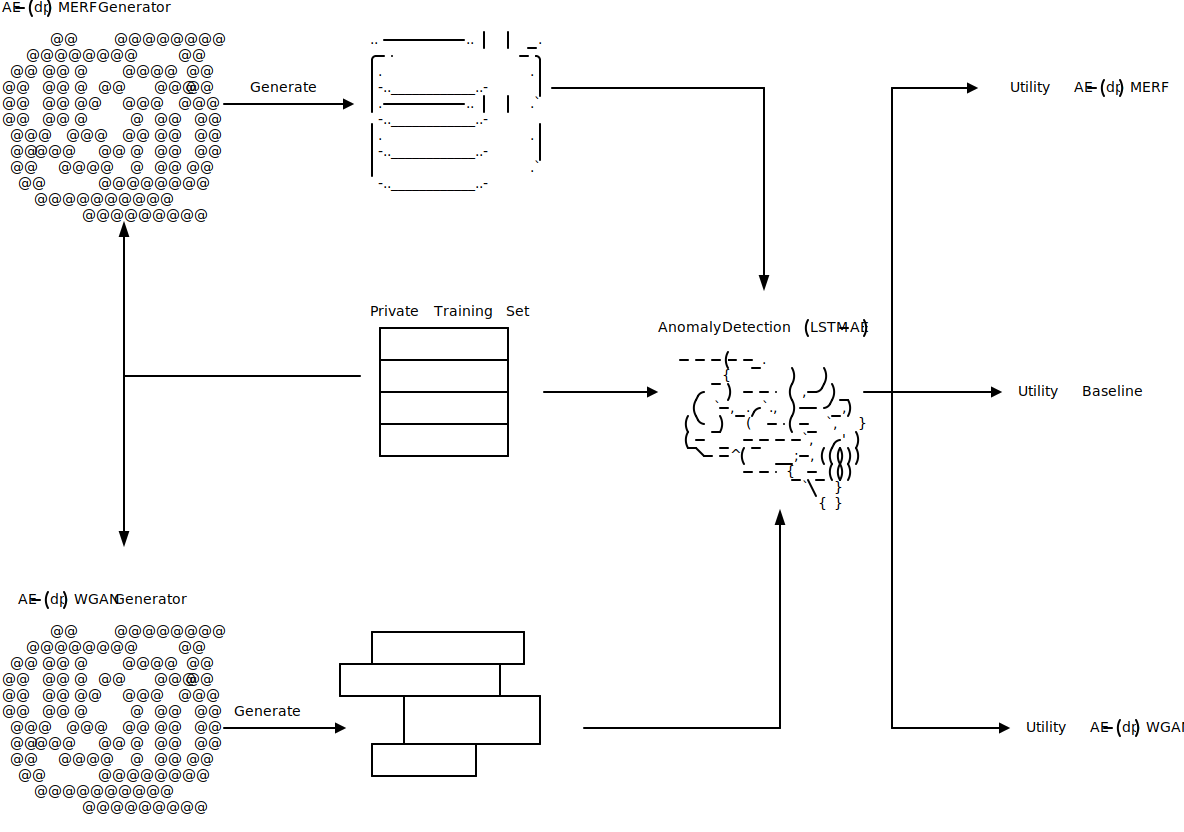
\includegraphics[scale=0.28]{str.png}
    \end{figure}
\end{frame}

\begin{frame}{Structure}
    \begin{enumerate}
        \item<1-> Train \alert{baseline model} for anomaly detection only on \alert{regular, private heartbeat data} using an LSTM-Autoencoder.
        \item<2->  \alert{Generate regular heartbeat} data using two approaches:
        \begin{itemize}
            \item<2-> [--] AE-(dp)MERF
            \item<2-> [--] AE-(dp)WGAN
        \end{itemize}
        \item<3->  Train LSTM-Autoencoder for \alert{anomaly detection on synthetic data} and \alert{test on real}.
        \item<3-> Assess \alert{utility} by measuring performance for anomaly detection (Accuracy, precision, recall, F1). 
        \item<4->  \alert{Contaminate} training data with anomalous heartbeats and repeat.
    \end{enumerate}
\end{frame}




\section{Dataset: MITBIH ECG data}
\begin{frame}{Heartbeat Arrhythmia}
    \begin{figure}
        \centering
        \includegraphics[scale=0.3]{images/heartbeat_arr.png}
        \caption[]{Different heartbeat arrhythmias \footnote{source: https://www.parkwayshenton.com.sg/health-plus/article/arrhythmia-guide}}
        \label{fig:enter-label}
    \end{figure}
\end{frame}

\begin{frame}{Arrhythmia Detection as an Anomaly Detection Problem}
We treat the problem of detecting anomalous heartbeats as an anomaly detection problem from machine learning based on the \alert{reconstruction error}:
\begin{itemize}
    \item<2->  We train a model \alert{on regular heartbeats} that is able to reconstruct that regular heartbeat.
    \item<3->  Given an anomalous heartbeat the model should give \alert{higher reconstruction error}.
    \item<4->  Based on an optimal \alert{threshold} for that error we classify this heartbeat as either regular or anomalous.
\end{itemize}
    \onslide<5>{Two reasons for this semi-supervised approach: high class imbalancy and no need for labelling.}
\end{frame} 

\begin{frame}{Baseline Model}
    Model is a LSTM-AE that is \alert{trained only on regular, private samples} with the goal to reconstruct normal samples. The classification is made based on the reconstruction error.
    \begin{columns}
        \begin{column}{0.48\textwidth}
        \begin{figure}
            \centering
            \includegraphics[scale=0.3]{images/rec_normal.png}
            \caption{reconstruction on normal sample \phantom{asdfsadf}}
            \label{fig:enter-label}
        \end{figure}
    \end{column}
    \begin{column}{0.48\textwidth}
        \begin{figure}
            \centering
            \includegraphics[scale=0.3]{images/rec_anom.png}
            \caption{reconstruction on anomalous sample}
            \label{fig:enter-label}
        \end{figure}
    \end{column}
    \end{columns}
\end{frame}



\section[(Time Series) Data generation]{(Time Series) Data generation}\label{chapter3}
\subsection{Overview}
    \begin{itemize}
        \item Data generation in general
        \item what is special about time series
        \item what about Privacy
        \item choice of models
    \end{itemize}

Time series data are sequences of data points in which there is a notion of time or ordering. Unlike tabular data, where each column corresponds to one feature, but it does not matter in which order one treats the different features. Time series are ubiquitous, common examples include weather data, financial transactions, energy consumption over time, stock prices etc.

We have chosen two architectures from the state of the art, that we will adapt to work on time series data. The first model is an example of a feature-based method, where a simple generative model is trained to map from a noise distribution to the data distribution. This is done by comparing the features of the synthetic data (or a suitable transformation thereof) with those of the original data. One particular instance of this class, DP-MERF \parencite{dpmerf}, has shown to give efficient and accurate results. Making this algorithm differentially private is straight-forward, since the loss function here can be separated into a term that is dependent on the original data and one that is not. So one only needs to introduce differential private noise to the data-dependent term once.


The second model follows a GAN-based approach. GANs introduced by Goodfellow et. al ???REF have been studied extensively in recent works as they have shown promising results in the field of image generation ??REF. They consist of two networks, a generator and a discriminator, where those two networks play a zero-sum game: the generator aims to generate authentic data whereas the discriminator aims to distinguish between generated and real data.


\subsection{DP-MERF}

DP-MERF \parencite{dpmerf} is an efficient all purpose data generation algorithm that is based on minimising the so-called Maximum Mean Discrepancy (MMD) between the real and the synthetic data distributions. It employs a so-called kernel mean embedding to transform the underlying probability distribution of the original data into a reproducing kernel hilbert space (RKHS). The distance between two distributions in the RKHS is then measured by the MMD. The authors mainly verified their results using tabular data like ????, but also image data, notably the MNIST ???CITE data set. It has not been used for time series data, but we will consider this data generation for generating time series data in this thesis, because according to a recent survey \parencite{hu2023sok}, DP-MERF delivers the best all purpose data generation performance.

\subsubsection{Maximum Mean Discrepancy}
There are different ways to measure the "distance" between two distributions $P$ and $Q$. On popular metric is the Maximum Mean Discrepancy (MMD) between $P$ and $Q$, where the random variables are projected into another feature space and the expected values are compared to each other in this space.

\begin{definition}[MMD]
    Let $\phi: \mathcal{X} \rightarrow \mathcal{H}$, where $\mathcal{H}$ is a reproducing kernel hilbert space (RKHS) and $P$ and $Q$ some distributions over $\mathcal{X}$ and random variables $X \sim P$, $Y \sim Q$ given. Then the Maximum mean Discrepancy is defined as:
    \begin{align}
        MMD(P,Q)=|| \mathbb{E}[\phi(X)] - \mathbb{E}[\phi(Y)] ||_\mathcal{H}
    \end{align}
\end{definition}

Some "easy" features maps $\phi$ are for example:
\begin{ex}
    Let $P$ and $Q$ some distributions over $\mathcal{X}$ and random variables $X \sim P$, $Y \sim Q$ given.
    \begin{itemize}
        \item \textbf{Identity kernel}: $\mathcal{X}=\mathcal{H}=\mathbb{R}^d$ and $\phi(x)=x$, then we have:
        \begin{align}
            MMD(P,Q) &= || \mathbb{E}[\phi(X)] - \mathbb{E}[\phi(Y)] ||_\mathcal{H} \nonumber \\
            &= || \mathbb{E}[X] - \mathbb{E}[Y] ||_{\mathbb{R}^d}
        \end{align}
        So we only compare the two distributions in terms of their means. 

        \item \textbf{Quadratic kernel}: $\mathcal{X}=\mathbb{R}$ $\mathcal{H}=\mathbb{R}^2$ and $\phi(x)=(x, x^2)$, then we have:
        \begin{align}
            MMD(P,Q) &= || \mathbb{E}[\phi(X)] - \mathbb{E}[\phi(Y)] ||_\mathcal{H} \nonumber \\
            &= || \mathbb{E}[(X, X^2)] - \mathbb{E}[(Y, Y^2)] ||_\mathcal{H} \nonumber \\
            &= || \begin{pmatrix}
                \mathbb{E}[X] \\ \mathbb{E}[X^2]
            \end{pmatrix} - \begin{pmatrix}
                \mathbb{E}[Y] \\ \mathbb{E}[Y^2]
            \end{pmatrix} ||_{\mathbb{R}^2} \nonumber \\
            &= \sqrt{(\mathbb{E}[X] - \mathbb{E}[Y])^2 - (\mathbb{E}[X^2] - \mathbb{E}[Y^2])^2}
        \end{align}
        So here we compare the two distributions in terms of their means and their variance (or first and second moments respectively).
        \item \textbf{Gaussian kernel} ????
    \end{itemize}
\end{ex}

Now instead of computing a possibly high or even infinite dimensional transformation $\phi$ one can use the well-known kernel trick ????REF. Let $k(x,y)=<\phi(x), \phi(y)>_{\mathcal{H}}$ be a kernel with corresponding reproducing kernel hilbert space $\mathcal{H}$, then the computation of the MMD simplifies to:

\begin{align}
    MMD^2(P,Q) &= || \mathbb{E}[\phi(X)] - \mathbb{E}[\phi(Y)] ||^2_\mathcal{H} \nonumber \\
    &= <\mathbb{E}[\phi(X)], \mathbb{E}[\phi(X')]> - <\mathbb{E}[\phi(X)], \mathbb{E}[\phi(Y)]> - <\mathbb{E}[\phi(Y)], \mathbb{E}[\phi(X)]> \nonumber \\ &\phantom{mmmmmmmmmmmmmmmmmmmm}+ <\mathbb{E}[\phi(Y)], \mathbb{E}[\phi(Y')]> \nonumber \\
    &= \mathbb{E}[<\phi(X), \phi(X')>] - 2 \mathbb{E}[<\phi(X), \phi(Y)>] + \mathbb{E}[<\phi(Y), \phi(Y')>] \nonumber \\
    &= \mathbb{E}[k(X,X')] - 2 \mathbb{E}[k(X,Y)] + \mathbb{E}[k(Y,Y')]
\end{align}

Where we introduced independent random variables $X,X' \sim P$, $Y,Y' \sim Q$.

\subsubsection{Random Fourier Features}

Now given a training data set $X_m = \{x_i\}_{i=1}^m \sim P$ and a synthetic data set $X'_m = \{x_i\}_{i=1}^m \sim Q$ we can estimate their $MMD^2$ by estimating the expected value with a mean estimate:

\begin{align} \label{eq:mmd}
    \widehat{MMD}^2(X_m, X'_m) = \frac{1}{m^2} \sum_{i,j=1}^m k(x_i,x_j) + \frac{1}{m^2} \sum_{i,j=1}^m k(x'_i,x'_j) - \frac{2}{m^2} \sum_{i,j=1}^m k(x_i,x'_j)
\end{align}
Unfortunately, this will require $\mathcal{O}(m^2)$ computations which grows quadratically in the number of samples. This will be too big for a large training data set. As a remedy, the authors of \parencite{dpmerf} propose to use Random Fourier Features based on a paper from 2007 \parencite[see][]{rff}, to approximate the kernel $k$ using its fourier transform and Monte-Carlo-Simulation.

\begin{align}
    k(x,y) \approx \hat{\Phi}(x)^T \hat{\Phi}(x')
\end{align}
where $\hat{\Phi}(x) \in \mathbb{R}^D$ and $\hat{\Phi}_j(x) = \sqrt{\frac{2}{D}} cos (\omega_j^T x)$.

If we sample $w_j \sim \mathcal{N}$ from the Gaussian distribution, we are approximating the gaussian kernel.

Now we can approximate equation \ref{eq:mmd} using those random fourier features:

\begin{align} \label{eq:rff}
    \widehat{MMD}^2_{RFF}(X_m, X'_m) &\approx \frac{1}{m^2} \sum_{i,j=1}^m \hat{\Phi}(x_i)^T \hat{\Phi}(x_j') + \frac{1}{m^2} \sum_{i,j=1}^m \hat{\Phi}(x_i)^T \hat{\Phi}(x_j') - \frac{2}{m^2} \sum_{i,j=1}^m \hat{\Phi}(x_i)^T \hat{\Phi}(x_j') \nonumber \\
    &= || \frac{1}{m} \sum_{i=1}^m \hat{\Phi}(x_i) - \frac{1}{m} \sum_{j=1}^m \hat{\Phi}(x_j') ||_\mathcal{H}^2
\end{align}

more stuff: https://gregorygundersen.com/blog/2019/12/23/random-fourier-features/

\subsubsection{Vanilla DP-MERF}
We can now introduce the version of DP-MERF presented in \parencite{dpmerf}. Let $G_\theta$ denote a generative neural network with parameters $\theta$, i.\ e.\ given input $z \sim p(z)$ from some known probability distribution $p(z)$ we obtain a synthetic sample through $x' = G_\theta(z)$. We denote the distribution of the synthetic data samples by $Q$. Further, let $X_m = \{x_i\}_{i=1}^m \sim P$ be our training data with true distribution $P$. By minimising 
\begin{align}
    \widehat{\theta} &= \argmin_\theta \widehat{MMD}^2_{RFF}(P, Q) \nonumber \\
    &\overset{\ref{eq:rff}}{=} \argmin_\theta || \frac{1}{m} \sum_{i=1}^m \hat{\Phi}(x_i) - \frac{1}{m} \sum_{j=1}^m \hat{\Phi}(x_j') ||_2^2 \nonumber \\
    &= \argmin_\theta || \hat{\mu}_P - \hat{\mu}_Q ||_2^2
\end{align}

where we introduced notation $\hat{\mu}_P = \frac{1}{m} \sum_{i=1}^m \hat{\Phi}(x_i)$ and $\hat{\mu}_Q = \frac{1}{m} \sum_{i=1}^m \hat{\Phi}(x'_i)$. The DP version is obtained by observing that the original data set is entering the equation only through $\hat{mu}_P$ so we have to introduce noise only in this term by adding gaussian noise:
\begin{align}
    \tilde{\mu}_p = \hat{\mu}_P + \mathcal{N}(0, \sigma^2 I)
\end{align}
We choose $\sigma$ according to definition \ref{def:gm}. For a given privacy level $(\epsilon, \delta)$ we need to compute the sensitivity $\Delta_{\hat{\mu}_P}$. There is an upper bound since we have by definition:
\begin{align}
    \Delta_{\hat{\mu}_P} &= \max_{\substack{X_m,X_m' \\ ||X_m-X_m'||_1=1}} || \frac{1}{m} \sum_{i=1}^m \hat{\Phi}(x_i) - \frac{1}{m} \sum_{j=1}^m \hat{\Phi}(x_j') ||_2 \nonumber \\
    &= \frac{1}{m} \max_{x_m \neq x'_m} || \hat{\Phi}(x_m) - \hat{\Phi}(x'_m)||_2 \nonumber \\
    &\overset{\Delta \neq}{\leq} \frac{1}{m} \max_{x_m \neq x'_m} || \hat{\Phi}(x_m) ||_2 + ||\hat{\Phi}(x'_m)||_2 \nonumber \\
    &\leq \frac{2}{m} 
\end{align}
where in the second equality we assumed without loss of generality that $X_m$ and $X_m'$ differ only in their last element, so that the other summands cancel each out and in the last inequality we are using the fact that $||\hat{\Phi}(\cdot)||_2 \leq 1$.


\subsection{GAN based} 

\section{Results}

\begin{frame}{AE-(DP)MERF}
    \begin{figure}
        \centering
        \includegraphics[scale=0.23]{results_aedpmerf.png}
        \caption{Results of AE-(DP)MERF with different privacy budgets (lower epsilon means higher privacy)}
        \label{fig:enter-label}
    \end{figure}
\end{frame}

\begin{frame}{(DP-)RTSGAN}
    \begin{figure}
        \centering
        \includegraphics[scale=0.23]{restuls_dprtsgan.png}
        \caption{Results of (DP-)RTSGAN with different privacy budgets (lower epsilon means higher privacy)}
        \label{fig:enter-label}
    \end{figure}
\end{frame}

\begin{frame}{Conclusion}
    \begin{itemize}
        \item DPMERF performs best and is very efficient computationally.
        \item DPMERF can work in lower epsilon ranges, which translates to higher privacy guarantees.
        \item DP-RTSGAN gives worse generative performance and can only work with meaningless privacy budgets epsilon.
        \item Adding privacy does not impact the utility for anomaly detection too much until too much noise is added.
    \end{itemize}
\end{frame}

\begin{frame}{Contamination}
    We contaminate the train set that only consists of normal samples with 1\%, 2\%, 5\% anomalous samples (the percentage of heartbeat arrhythmias is estimated to be around max. 5\%).
\end{frame}

\begin{frame}{Contamination: AE-(DP)MERF}
    \begin{figure}
        \centering
        \includegraphics[scale=0.33]{results_aedpmerf_contam.png}
        \caption{Contaminated training set: AE-(DP)MERF}
        \label{fig:enter-label}
    \end{figure}
\end{frame}



\section{Summary}
\begin{frame}{Summary}
    \begin{itemize}
        \item<1-> We tested two different \alert{DP times series data generation} models on the MITBIH ECG data set.
        \item<2-> We measured the \alert{utility} of the synthetic data via the downstream task of anomaly detection (heartbeat arrhythmia).
        \item<3-> We investigated the \alert{robustness} of the data generation by \alert{contaminating} the data set with anomalous samples.
    \end{itemize}
\end{frame}

\begin{frame}
    \frametitle{Main Findings}
        \begin{itemize}
            \item<1-> AE-(dp)MERF works better than GAN based approach.
            \item<2-> The \alert{Privacy-Utility-Tradeoff is more nuanced} and depends on the use case. For anomaly detection, privacy and utility can go hand in hand.
            \item<3-> Synthetic data and DP can add \alert{robustness}.
        \end{itemize}
\end{frame}

\begin{frame}
    \frametitle{Future Work}
    \begin{itemize}
        \item<1-> Test with \alert{other time series data}.
        \item<2-> Work with \alert{other use cases}, e.g. classification, regression.
        \item<3-> Further investigate \alert{robustness}.
        \item<4-> Verify theoretical privacy guarantees with empirical tests, e.g. \alert{membership inference attacks}.
    \end{itemize}
\end{frame}

\begin{frame}
    \frametitle{Privacy-Preserving Acknowledgement}

    \huge
    Thank you Aflsono, Apslotsuo, Hna, Sihahd!
    

\end{frame}

\section{References}
\begin{frame}[allowframebreaks]{}
    % Beamer does not support BibTeX so references must be inserted manually as below
    \nocite{*}
    \printbibliography
\end{frame}


\section*{Backup}

\begin{frame}
    \frametitle{}
    \centering
    \huge
    \alert{$>>>$ BACKUP}

\end{frame}

\begin{frame}
    \frametitle{Model Architecture}

    

\end{frame}

\end{document}